\documentclass[10pt,twocolumn,letterpaper]{article}

\usepackage{eso-pic}
\usepackage{cvpr}
\usepackage{times}
\usepackage{epsfig}
\usepackage{graphicx}
\usepackage{amsmath}
\usepackage{amssymb}


% Include other packages here, before hyperref.
\usepackage{my_macros}
%\usepackage{framed}
\usepackage{caption}
\usepackage{subcaption}
%for tikz
\usepackage{tikz,pgfplots}
\usetikzlibrary{arrows,positioning,automata,shadows,fit,shapes}
\usetikzlibrary{arrows,petri,topaths}
\usetikzlibrary{positioning,fit,calc}
\usetikzlibrary{shapes.arrows,chains,decorations.pathreplacing,fadings}
\usepackage{tkz-berge}

\definecolor{shadecolor}{rgb}{0.01,0.199,0.1}

% If you comment hyperref and then uncomment it, you should delete
% egpaper.aux before re-running latex.  (Or just hit 'q' on the first latex
% run, let it finish, and you should be clear).
\usepackage[pagebackref=true,breaklinks=true,letterpaper=true,colorlinks,bookmarks=false]{hyperref}

% \cvprfinalcopy % *** Uncomment this line for the final submission

\def\cvprPaperID{****} % *** Enter the CVPR Paper ID here
\def\httilde{\mbox{\tt\raisebox{-.5ex}{\symbol{126}}}}

% Pages are numbered in submission mode, and unnumbered in camera-ready
\ifcvprfinal\pagestyle{empty}\fi
\begin{document}
%%%%%%%%% TITLE
%!TEX root = egpaper_for_review.tex
\newcommand{\Cut }{\mathcal{C}}
\title{FancyMc Moves \\ Fusion Moves for Multicut Objectives}

\author{First Author\\
Institution1\\
Institution1 address\\
{\tt\small firstauthor@i1.org}
% For a paper whose authors are all at the same institution,
% omit the following lines up until the closing ``}''.
% Additional authors and addresses can be added with ``\and'',
% just like the second author.
% To save space, use either the email address or home page, not both
\and
Second Author\\
Institution2\\
First line of institution2 address\\
{\tt\small secondauthor@i2.org}
}

\maketitle
%\thispagestyle{empty}

%%%%%%%%% ABSTRACT
\begin{abstract}
   Multicuts rule.
\end{abstract}
\section{Introduction}

The tale of the multicut

%-------------------------------------------------------------------------

\subsection{Related Work}

\subsubsection{Multicut}
   \begin{itemize}
   \item Andres \etal~\cite{andres_2011_iccv}
   \item Kappes \etal~\cite{kappes_2011_emmcvpr}
   \item Bagon and Galun~\cite{bagon_2011_arxiv}
   \item Yarkony \etal~\cite{yarkony_2012_eccv}
   \item Beier \etal~\cite{beier_2014_cvpr}
   \end{itemize}

\subsubsection{Fusion Moves}
Move making algorithms, in particular fusion moves, 
have become increasingly popular for energy minimization~\cite{???,kappes_2014_ws}.
For many large scale computer vision applications fusion moves lead to good approximations
with state of the art any time performance~\cite{kappes_2014_ws}.








%------------------------------------------------------------------------
\section{Name of My Method (Union Fusion Cut)}

Global optimal solvers for multicut do not scale beyond ??? \cite{???}.
Good approximate solvers for planar graphs exist \cite{beier_2014_cvpr,yarkony_2012_eccv} 
but have difficulties to find good solutions for non planar graphs \cite{beier_2014_cvpr}.



%!TEX root = egpaper_for_review.tex
\begin{figure}[H]

\tikzfading[name=fade right0,left color=transparent!0, right color=transparent!70]
\tikzfading[name=fade right1,left color=transparent!70, right color=transparent!100]
\tikzstyle{gNode}=[fill=white,draw,solid,font=\sffamily\small]
\tikzstyle{cutNode}=[fill=white,draw,solid,font=\sffamily\small]
\tikzstyle{opBox}=[fill=black,text=white,draw,solid,font=\sffamily\tiny,align=center]
\tikzstyle{label}=[fill=black,text=white,draw,solid,font=\sffamily\tiny]
\tikzstyle{edgeLabelNode}=[ellipse,text=black,solid,font=\sffamily\tiny,align=left,minimum size=0.5cm]
\tikzstyle{aEdge}=[->,node distance=0.5cm]
\begin{tikzpicture}
    
    \draw node[opBox] (gen) {GENERATOR};
    \draw node[cutNode,right = 1cm of gen] (proposal_cut) {$\bar{P}$};
    \draw node[right of = proposal_cut](dummy){};
    \draw node[cutNode,right of = dummy] (best_cut) {$P$};
    \draw node[opBox,below of = dummy] (intersect) {INTERSECT\\UNCUT};
    \draw node[cutNode,below of = intersect] (int_cut){$\tilde{P}$};
    \draw node[opBox,below of = int_cut] (contract) {CONTRACT\\UNCUT\\EDGES};
    \draw node[gNode,right = 2cm of contract](cgraph)  {$( \tilde{\mathcal{G}}, \tilde{\mathcal{W}})$};
    \draw node[opBox, above of =  cgraph] (multicut) {MULTICUT};
    \draw node[cutNode,above of = multicut] (rcut) {$\bar{P}^{\tilde{\mathcal{G}}}$};
    \draw node[opBox, above of =  rcut] (pback) {PROJECT\\CUT\\BACK};

    \node[draw,dotted,fit=(proposal_cut) (cgraph),inner sep = 3mm,thick, draw=gray,opacity=0.5] {};

    \draw node[gNode,below = of gen](graph)  {$( \mathcal{G}, \mathcal{W})$};
    \path[]
    (gen) edge[aEdge]  node[]{} (proposal_cut)
    (graph) edge[aEdge] (gen)
    (proposal_cut)  edge[aEdge]   (intersect)
    (best_cut)      edge[aEdge]   (intersect)
    (intersect)     edge[aEdge]   (int_cut)
    (int_cut)       edge[aEdge]   (contract) 
    (contract)      edge[aEdge,above]   
        node[edgeLabelNode]{coarse graphs\\with fewer nodes}(cgraph)
    (cgraph)        edge[aEdge]   (multicut)
    (multicut)      edge[aEdge]   (rcut)
    (rcut)          edge[aEdge]   (pback)
    (pback)         edge[aEdge]   (best_cut)
    (graph)         edge[aEdge]   (contract.west)
    (best_cut)      edge[aEdge,dashed,bend angle=90,bend right,draw=gray!30]  
        node[edgeLabelNode]{current best solution\\can influence generator}  (gen)
    ;
\end{tikzpicture}
\caption{
    The proposed algorithm works in the following way:
    Given a graph $\mathcal{G}$, edge weights $\mathcal{W}$ and
    a proposal generator, the current best solution $P$ is iteratively improved.
    A proposal generator generates different versatile
    proposal partitions $\bar{P}$.
    The proposal  $\bar{P}$ is intersected with $P$ which results in
    $\tilde{P}$. Contracting each each which is not 
    cut in $\tilde{P}$ leads to a coarser graph  
    $\tilde{\mathcal{G}} = ( \tilde{\mathcal{V}}, \tilde{\mathcal{E}} )$ 
    with new edge weights $\tilde{\mathcal{W}}$.
    If  $\bar{P}$ and $P$ have a small fraction of cut edges, $\tilde{\mathcal{G}}$ will be small ( $|\tilde{\mathcal{V}}| << |\mathcal{V}|$
    and $|\tilde{\mathcal{E}}| << |\mathcal{E}|$).
    The multicut objective on the smaller graph $\tilde{\mathcal{G}}$ can be optimized magnitudes 
    faster than on $\tilde{\mathcal{G}}$.
    It is guaranteed that the optimal multicut partitioning $\bar{P}^{\tilde{\mathcal{G}}}$ on $\tilde{\mathcal{G}}$ projected 
    back to $\mathcal{G}$ as a lower or equal energy than any of the two input partitions $P$ and $\bar{P}$, 
    therefore we store the result of fusion as new best state $P$ and repeat the procedure.
}\label{fig:algo_graph}
\end{figure}


\begin{figure}[H]

\begin{tikzpicture}
    \tikzstyle{pixel}=[regular polygon,regular polygon sides=4,inner sep=0pt,draw,solid,font=\sffamily\small]

    \node[anchor=south west,inner sep=0] (image) at (0,0) {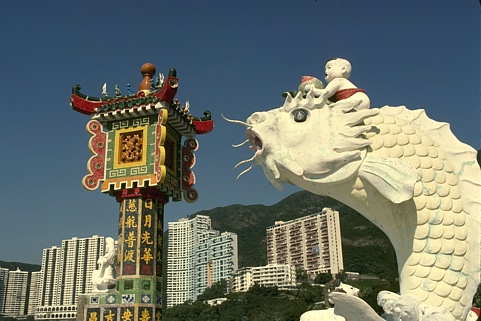
\includegraphics[width=.25\textwidth]{images/120093.jpg}};
    \begin{scope}[x={(image.south east)},y={(image.north west)}]
        \draw[red,ultra thick,rounded corners] (0.62,0.65) rectangle (0.78,0.75);
        \draw node[pixel ](100.5,100.5) {BLAAA};
    \end{scope}
\end{tikzpicture}



\end{figure}

%!TEX root = egpaper_for_review.tex
\begin{figure*}
\tikzstyle{cedge}=[fill=white,dotted,font=\sffamily\tiny, opacity=0.5, text=gray]
\tikzstyle{aedge}=[fill=white,solid,font=\sffamily\tiny, text=black!70          ]
\tikzstyle{vert}=[circle,minimum size = 0.5cm,inner sep = 1pt,draw, font=\small,align=left]
\centering
\begin{subfigure}[t]{0.20\linewidth}
   %\begin{framed}
   \resizebox{1.0\linewidth}{!}{
      \begin{tikzpicture}[scale=1.0,transform shape]
        \tikzstyle{vert}=[circle,minimum size = 0.5cm,inner sep = 0pt,draw, font=\small, node distance = 5cm]
        \draw (0*2,3*2) node[vert](1){$1$};
        \draw (1*2,3*2) node[vert](2){$2$};
        \draw (2*2,3*2) node[vert](3){$3$};
        \draw (3*2,3*2) node[vert](4){$4$};
        \draw (0*2,2*2) node[vert](5){$5$};
        \draw (1*2,2*2) node[vert](6){$6$};
        \draw (2*2,2*2) node[vert](7){$7$};
        \draw (3*2,2*2) node[vert](8){$8$};
        \draw (0*2,1*2) node[vert](9){$9$};
        \draw (1*2,1*2) node[vert](10){$10$};
        \draw (2*2,1*2) node[vert](11){$11$};
        \draw (3*2,1*2) node[vert](12){$12$};
        \draw (0*2,0*2) node[vert](13){$13$};
        \draw (1*2,0*2) node[vert](14){$14$};
        \draw (2*2,0*2) node[vert](15){$15$};
        \draw (3*2,0*2) node[vert](16){$16$};
        %
        \path[every node/.style={font=\sffamily\tiny, fill=white}]
            (1)     edge[aedge]     node{$w_{(1, 2)}$   }     (2)
            (2)     edge[aedge]     node{$w_{(2, 3)}$   }     (3)
            (3)     edge[aedge]     node{$w_{(3, 4)}$   }     (4)
            (5)     edge[aedge]     node{$w_{(5, 6)}$   }     (6)
            (6)     edge[aedge]     node{$w_{(6, 7)}$   }     (7)
            (7)     edge[aedge]     node{$w_{(7, 8)}$   }     (8)
            (9)     edge[aedge]     node{$w_{(9, 10)}$  }     (10)
            (10)    edge[aedge]     node{$w_{(10, 11)}$ }     (11)
            (11)    edge[aedge]     node{$w_{(11, 12)}$ }     (12)
            (13)    edge[aedge]     node{$w_{(13, 14)}$ }     (14)
            (14)    edge[aedge]     node{$w_{(14, 15)}$ }     (15)
            (15)    edge[aedge]     node{$w_{(15, 16)}$ }     (16)
            (1)     edge[aedge]     node{$w_{(1, 5)}$   }     (5)
            (5)     edge[aedge]     node{$w_{(5, 9)}$   }     (9)
            (9)     edge[aedge]     node{$w_{(9, 13)}$  }     (13)
            (2)     edge[aedge]     node{$w_{(2, 6)}$   }     (6)
            (6)     edge[aedge]     node{$w_{(6, 10)}$  }     (10)
            (10)    edge[aedge]     node{$w_{(10, 14)}$ }     (14)
            (3)     edge[aedge]     node{$w_{(3, 7)}$   }     (7)
            (7)     edge[aedge]     node{$w_{(7, 11)}$  }     (11)
            (11)    edge[aedge]     node{$w_{(11, 15)}$ }     (15)
            (4)     edge[aedge]     node{$w_{(4, 8)}$   }     (8)
            (8)     edge[aedge]     node{$w_{(8, 12)}$  }     (12)
            (12)    edge[aedge]     node{$w_{(12, 16)}$ }     (16)
        ;
      \end{tikzpicture}
   }
   %\end{framed} 
\caption{Graph $\mathcal{G}$}    
\end{subfigure}\quad\quad
\begin{subfigure}[t]{0.20\linewidth}
   %\begin{framed}
   \resizebox{1.0\linewidth}{!}{
      \begin{tikzpicture}[scale=1.0,transform shape]

        \draw (0*2,3*2) node[vert,fill=red!50](1){$1$};
        \draw (1*2,3*2) node[vert,fill=red!50](2){$2$};
        \draw (2*2,3*2) node[vert,fill=red!50](3){$3$};
        \draw (3*2,3*2) node[vert,fill=red!50](4){$4$};
        \draw (0*2,2*2) node[vert,fill=red!50](5){$5$};
        \draw (1*2,2*2) node[vert,fill=red!50](6){$6$};
        \draw (2*2,2*2) node[vert,fill=red!50](7){$7$};
        \draw (3*2,2*2) node[vert,fill=red!50](8){$8$};
        \draw (0*2,1*2) node[vert,fill=blue!50](9){$9$};
        \draw (1*2,1*2) node[vert,fill=blue!50](10){$10$};
        \draw (2*2,1*2) node[vert,fill=blue!50](11){$11$};
        \draw (3*2,1*2) node[vert,fill=blue!50](12){$12$};
        \draw (0*2,0*2) node[vert,fill=blue!50](13){$13$};
        \draw (1*2,0*2) node[vert,fill=blue!50](14){$14$};
        \draw (2*2,0*2) node[vert,fill=blue!50](15){$15$};
        \draw (3*2,0*2) node[vert,fill=blue!50](16){$16$};
        %
        \path[every node/.style={font=\sffamily\tiny, fill=white}]
            (1)     edge[aedge]     node{$w_{(1, 2)}$   }     (2)
            (2)     edge[aedge]     node{$w_{(2, 3)}$   }     (3)
            (3)     edge[aedge]     node{$w_{(3, 4)}$   }     (4)
            (5)     edge[aedge]     node{$w_{(5, 6)}$   }     (6)
            (6)     edge[aedge]     node{$w_{(6, 7)}$   }     (7)
            (7)     edge[aedge]     node{$w_{(7, 8)}$   }     (8)
            (9)     edge[aedge]     node{$w_{(9, 10)}$  }     (10)
            (10)    edge[aedge]     node{$w_{(10, 11)}$ }     (11)
            (11)    edge[aedge]     node{$w_{(11, 12)}$ }     (12)
            (13)    edge[aedge]     node{$w_{(13, 14)}$ }     (14)
            (14)    edge[aedge]     node{$w_{(14, 15)}$ }     (15)
            (15)    edge[aedge]     node{$w_{(15, 16)}$ }     (16)
            (1)     edge[aedge]     node{$w_{(1, 5)}$   }     (5)
            (5)     edge[cedge]     node{$w_{(5, 9)}$   }     (9)
            (9)     edge[aedge]     node{$w_{(9, 13)}$  }     (13)
            (2)     edge[aedge]     node{$w_{(2, 6)}$   }     (6)
            (6)     edge[cedge]     node{$w_{(6, 10)}$  }     (10)
            (10)    edge[aedge]     node{$w_{(10, 14)}$ }     (14)
            (3)     edge[aedge]     node{$w_{(3, 7)}$   }     (7)
            (7)     edge[cedge]     node{$w_{(7, 11)}$  }     (11)
            (11)    edge[aedge]     node{$w_{(11, 15)}$ }     (15)
            (4)     edge[aedge]     node{$w_{(4, 8)}$   }     (8)
            (8)     edge[cedge]     node{$w_{(8, 12)}$  }     (12)
            (12)    edge[aedge]     node{$w_{(12, 16)}$ }     (16)
        ;
      \end{tikzpicture}
   }
   %\end{framed}
\caption{$\mathcal{E}^A_{cut}$}
\end{subfigure}\quad\quad
\begin{subfigure}[t]{0.20\linewidth}
   %\begin{framed}
   \resizebox{1.0\linewidth}{!}{
      \begin{tikzpicture}[scale=1.0,transform shape]

        \draw (0*2,3*2) node[vert,fill=green!50](1){$1$};
        \draw (1*2,3*2) node[vert,fill=orange!50](2){$2$};
        \draw (2*2,3*2) node[vert,fill=orange!50](3){$3$};
        \draw (3*2,3*2) node[vert,fill=orange!50](4){$4$};
        \draw (0*2,2*2) node[vert,fill=yellow!=30](5){$5$};
        \draw (1*2,2*2) node[vert,fill=magenta!40](6){$6$};
        \draw (2*2,2*2) node[vert,fill=magenta!40](7){$7$};
        \draw (3*2,2*2) node[vert,fill=magenta!40](8){$8$};
        \draw (0*2,1*2) node[vert,fill=yellow!=30](9){$9$};
        \draw (1*2,1*2) node[vert,fill=magenta!40](10){$10$};
        \draw (2*2,1*2) node[vert,fill=magenta!40](11){$11$};
        \draw (3*2,1*2) node[vert,fill=magenta!40](12){$12$};
        \draw (0*2,0*2) node[vert,fill=yellow!=30](13){$13$};
        \draw (1*2,0*2) node[vert,fill=magenta!40](14){$14$};
        \draw (2*2,0*2) node[vert,fill=magenta!40](15){$15$};
        \draw (3*2,0*2) node[vert,fill=magenta!40](16){$16$};
        %
        \path[every node/.style={font=\sffamily\tiny, fill=white}]
            (1)     edge[cedge]     node{$w_{(1, 2)}$   }     (2)
            (2)     edge[aedge]     node{$w_{(2, 3)}$   }     (3)
            (3)     edge[aedge]     node{$w_{(3, 4)}$   }     (4)
            (5)     edge[cedge]     node{$w_{(5, 6)}$   }     (6)
            (6)     edge[aedge]     node{$w_{(6, 7)}$   }     (7)
            (7)     edge[aedge]     node{$w_{(7, 8)}$   }     (8)
            (9)     edge[cedge]     node{$w_{(9, 10)}$  }     (10)
            (10)    edge[aedge]     node{$w_{(10, 11)}$ }     (11)
            (11)    edge[aedge]     node{$w_{(11, 12)}$ }     (12)
            (13)    edge[cedge]     node{$w_{(13, 14)}$ }     (14)
            (14)    edge[aedge]     node{$w_{(14, 15)}$ }     (15)
            (15)    edge[aedge]     node{$w_{(15, 16)}$ }     (16)
            (1)     edge[cedge]     node{$w_{(1, 5)}$   }     (5)
            (5)     edge[aedge]     node{$w_{(5, 9)}$   }     (9)
            (9)     edge[aedge]     node{$w_{(9, 13)}$  }     (13)
            (2)     edge[cedge]     node{$w_{(2, 6)}$   }     (6)
            (6)     edge[aedge]     node{$w_{(6, 10)}$  }     (10)
            (10)    edge[aedge]     node{$w_{(10, 14)}$ }     (14)
            (3)     edge[cedge]     node{$w_{(3, 7)}$   }     (7)
            (7)     edge[aedge]     node{$w_{(7, 11)}$  }     (11)
            (11)    edge[aedge]     node{$w_{(11, 15)}$ }     (15)
            (4)     edge[cedge]     node{$w_{(4, 8)}$   }     (8)
            (8)     edge[aedge]     node{$w_{(8, 12)}$  }     (12)
            (12)    edge[aedge]     node{$w_{(12, 16)}$ }     (16)
        ;
      \end{tikzpicture}
   }
   %\end{framed}
\caption{$\mathcal{E}^B_{cut}$}  
\end{subfigure}\quad\quad
\begin{subfigure}[t]{0.20\linewidth}
   %\begin{framed}
   \resizebox{1.0\linewidth}{!}{
      \begin{tikzpicture}[scale=1.0,transform shape]

        \draw (0*2,3*2) node[vert,fill=blue!50!green](1){$1$};
        \draw (1*2,3*2) node[vert,fill=brown!50](2){$2$};
        \draw (2*2,3*2) node[vert,fill=brown!50](3){$3$};
        \draw (3*2,3*2) node[vert,fill=brown!50](4){$4$};
        \draw (0*2,2*2) node[vert,fill=cyan!=30](5){$5$};
        \draw (1*2,2*2) node[vert,fill=red!50!lime](6){$6$};
        \draw (2*2,2*2) node[vert,fill=red!50!lime](7){$7$};
        \draw (3*2,2*2) node[vert,fill=red!50!lime](8){$8$};
        \draw (0*2,1*2) node[vert,fill=violet!60](9){$9$};
        \draw (1*2,1*2) node[vert,fill=lime!40](10){$10$};
        \draw (2*2,1*2) node[vert,fill=lime!40](11){$11$};
        \draw (3*2,1*2) node[vert,fill=lime!40](12){$12$};
        \draw (0*2,0*2) node[vert,fill=violet!60](13){$13$};
        \draw (1*2,0*2) node[vert,fill=lime!40](14){$14$};
        \draw (2*2,0*2) node[vert,fill=lime!40](15){$15$};
        \draw (3*2,0*2) node[vert,fill=lime!40](16){$16$};
        %
        \path[every node/.style={font=\sffamily\tiny, fill=white}]
            (1)     edge[cedge]     node{$w_{(1, 2)}$   }     (2)
            (2)     edge[aedge]     node{$w_{(2, 3)}$   }     (3)
            (3)     edge[aedge]     node{$w_{(3, 4)}$   }     (4)
            (5)     edge[cedge]     node{$w_{(5, 6)}$   }     (6)
            (6)     edge[aedge]     node{$w_{(6, 7)}$   }     (7)
            (7)     edge[aedge]     node{$w_{(7, 8)}$   }     (8)
            (9)     edge[cedge]     node{$w_{(9, 10)}$  }     (10)
            (10)    edge[aedge]     node{$w_{(10, 11)}$ }     (11)
            (11)    edge[aedge]     node{$w_{(11, 12)}$ }     (12)
            (13)    edge[cedge]     node{$w_{(13, 14)}$ }     (14)
            (14)    edge[aedge]     node{$w_{(14, 15)}$ }     (15)
            (15)    edge[aedge]     node{$w_{(15, 16)}$ }     (16)
            (1)     edge[cedge]     node{$w_{(1, 5)}$   }     (5)
            (5)     edge[cedge]     node{$w_{(5, 9)}$   }     (9)
            (9)     edge[aedge]     node{$w_{(9, 13)}$  }     (13)
            (2)     edge[cedge]     node{$w_{(2, 6)}$   }     (6)
            (6)     edge[cedge]     node{$w_{(6, 10)}$  }     (10)
            (10)    edge[aedge]     node{$w_{(10, 14)}$ }     (14)
            (3)     edge[cedge]     node{$w_{(3, 7)}$   }     (7)
            (7)     edge[cedge]     node{$w_{(7, 11)}$  }     (11)
            (11)    edge[aedge]     node{$w_{(11, 15)}$ }     (15)
            (4)     edge[cedge]     node{$w_{(4, 8)}$   }     (8)
            (8)     edge[cedge]     node{$w_{(8, 12)}$  }     (12)
            (12)    edge[aedge]     node{$w_{(12, 16)}$ }     (16)
        ;
      \end{tikzpicture}
   }
   %\end{framed}
\caption{$\mathcal{E}^{AB}_{cut} = \mathcal{E}^B_{cut} \cup \mathcal{E}^B_{cut}$}  
\end{subfigure}

\vspace{0.1cm}

\begin{subfigure}[t]{0.20\linewidth}
   %\begin{framed}
   \resizebox{1.0\linewidth}{!}{
      \begin{tikzpicture}[scale=1.0,transform shape]
        \draw (0*2,3*2) node[vert](1){$\{1\}$};
        \draw (2*2,3*2) node[vert](2){$\{2, 3, 4\}$};
        \draw (0*2,2*2) node[vert,](5){$\{5\}$};
        \draw (2*2,2*2) node[vert](6){$\{6, 7, 8\}$};
        \draw (0*2,1*2) node[vert](9){$\{9, 13\}$};
        \draw (2*2,0.811*2) node[vert ](10){$\{10, 11, 12,$\\$14, 15, 16\}$};
        %
        \path[every node/.style={font=\sffamily\tiny, fill=white}]
            (1)     edge[aedge]     node{$w_{(1, 2)}$   }     (2)
            (1)     edge[aedge]     node{$w_{(1, 5)}$   }     (5)
            (1)     edge[aedge]     node{$w_{(1, 5)}$   }     (5)
            (5)     edge[aedge]     node{$w_{(5, 6)}$   }     (6)
            (5)     edge[aedge]     node{$w_{(5, 9)}$   }     (9)
            (9)     edge[aedge]     node{$w_{(9, 10)} + w_{(13, 14)}$   }     (10)
            (2)     edge[aedge]     node{$w_{(2, 6)} + w_{(3, 7)} + w_{(4, 8)} $   }     (6)
            (6)     edge[aedge]     node{$w_{(6, 10)} + w_{(7, 11)} + w_{(8, 12)} $   }     (10)
        ;
        %;
      \end{tikzpicture}
   }
   %\end{framed}
\caption{$\mathcal{\bar{G}}=\textbf{\scriptsize{contract}}(\mathcal{E} \backslash \{\mathcal{E}^{AB}_{cut}\})$}
\end{subfigure}
\quad\quad\quad
\begin{subfigure}[t]{0.20\linewidth}
   %\begin{framed}
   \resizebox{1.0\linewidth}{!}{
      \begin{tikzpicture}[scale=1.0,transform shape]
        \draw (0*2,3*2) node[vert,fill=blue!20!cyan](1){$\{1\}$};
        \draw (2*2,3*2) node[vert,fill=green!30!cyan](2){$\{2, 3, 4\}$};
        \draw (0*2,2*2) node[vert,fill=blue!20!cyan ](5){$\{5\}$};
        \draw (2*2,2*2) node[vert,fill=blue!40!green](6){$\{6, 7, 8\}$};
        \draw (0*2,1*2) node[vert,fill=blue!40!green](9){$\{9, 13\}$};
        \draw (2*2,0.811*2) node[vert,fill=blue!40!green](10){$\{10, 11, 12,$\\$14, 15, 16\}$};
        %
        \path[every node/.style={font=\sffamily\tiny, fill=white}]
            (1)     edge[cedge]     node{$w_{(1, 2)}$   }     (2)
            (1)     edge[cedge]     node{$w_{(1, 5)}$   }     (5)
            (1)     edge[aedge]     node{$w_{(1, 5)}$   }     (5)
            (5)     edge[cedge]     node{$w_{(5, 6)}$   }     (6)
            (5)     edge[cedge]     node{$w_{(5, 9)}$   }     (9)
            (9)     edge[aedge]     node{$w_{(9, 10)} + w_{(13, 14)}$   }     (10)
            (2)     edge[cedge]     node{$w_{(2, 6)} + w_{(3, 7)} + w_{(4, 8)} $   }     (6)
            (6)     edge[aedge]     node{$w_{(6, 10)} + w_{(7, 11)} + w_{(8, 12)} $   }     (10)
        ;
        %;
      \end{tikzpicture}
   }
   %\end{framed}
\caption{$\mathcal{E}_{\textit{\tiny{cut}}}^{\bar{\mathcal{G}}}  $}
\end{subfigure}
\quad\quad\quad
\begin{subfigure}[t]{0.20\linewidth}
   %\begin{framed}
   \resizebox{1.0\linewidth}{!}{
      \begin{tikzpicture}[scale=1.0,transform shape]

        \draw (0*2,3*2) node[vert,fill=blue!20!cyan](1){$1$};
        \draw (1*2,3*2) node[vert,fill=green!30!cyan](2){$2$};
        \draw (2*2,3*2) node[vert,fill=green!30!cyan](3){$3$};
        \draw (3*2,3*2) node[vert,fill=green!30!cyan](4){$4$};
        \draw (0*2,2*2) node[vert,fill=blue!20!cyan](5){$5$};
        \draw (1*2,2*2) node[vert,fill=blue!40!green](6){$6$};
        \draw (2*2,2*2) node[vert,fill=blue!40!green](7){$7$};
        \draw (3*2,2*2) node[vert,fill=blue!40!green](8){$8$};
        \draw (0*2,1*2) node[vert,fill=blue!40!green](9){$9$};
        \draw (1*2,1*2) node[vert,fill=blue!40!green](10){$10$};
        \draw (2*2,1*2) node[vert,fill=blue!40!green](11){$11$};
        \draw (3*2,1*2) node[vert,fill=blue!40!green](12){$12$};
        \draw (0*2,0*2) node[vert,fill=blue!40!green](13){$13$};
        \draw (1*2,0*2) node[vert,fill=blue!40!green](14){$14$};
        \draw (2*2,0*2) node[vert,fill=blue!40!green](15){$15$};
        \draw (3*2,0*2) node[vert,fill=blue!40!green](16){$16$};
        %
        \path[every node/.style={font=\sffamily\tiny, fill=white}]
            (1)     edge[cedge]     node{$w_{(1, 2)}$   }     (2)
            (2)     edge[aedge]     node{$w_{(2, 3)}$   }     (3)
            (3)     edge[aedge]     node{$w_{(3, 4)}$   }     (4)
            (5)     edge[cedge]     node{$w_{(5, 6)}$   }     (6)
            (6)     edge[aedge]     node{$w_{(6, 7)}$   }     (7)
            (7)     edge[aedge]     node{$w_{(7, 8)}$   }     (8)
            (9)     edge[aedge]     node{$w_{(9, 10)}$  }     (10)
            (10)    edge[aedge]     node{$w_{(10, 11)}$ }     (11)
            (11)    edge[aedge]     node{$w_{(11, 12)}$ }     (12)
            (13)    edge[aedge]     node{$w_{(13, 14)}$ }     (14)
            (14)    edge[aedge]     node{$w_{(14, 15)}$ }     (15)
            (15)    edge[aedge]     node{$w_{(15, 16)}$ }     (16)
            (1)     edge[aedge]     node{$w_{(1, 5)}$   }     (5)
            (5)     edge[cedge]     node{$w_{(5, 9)}$   }     (9)
            (9)     edge[aedge]     node{$w_{(9, 13)}$  }     (13)
            (2)     edge[cedge]     node{$w_{(2, 6)}$   }     (6)
            (6)     edge[aedge]     node{$w_{(6, 10)}$  }     (10)
            (10)    edge[aedge]     node{$w_{(10, 14)}$ }     (14)
            (3)     edge[cedge]     node{$w_{(3, 7)}$   }     (7)
            (7)     edge[aedge]     node{$w_{(7, 11)}$  }     (11)
            (11)    edge[aedge]     node{$w_{(11, 15)}$ }     (15)
            (4)     edge[cedge]     node{$w_{(4, 8)}$   }     (8)
            (8)     edge[aedge]     node{$w_{(8, 12)}$  }     (12)
            (12)    edge[aedge]     node{$w_{(12, 16)}$ }     (16)
        ;
      \end{tikzpicture}
   }
   %\end{framed}
\caption{$\mathcal{E}_{\textit{\tiny{cut}}}^{\bar{\mathcal{G}}}=\textbf{\scriptsize{projectBack}} (\mathcal{E}_{\textit{\tiny{cut}}}^{\bar{\mathcal{G}}} )  $}
\end{subfigure}
\caption{
        Describe Method here
}
\end{figure*}




%-------------------------------------------------------------------------
\subsection{Proposal Generators}



%-------------------------------------------------------------------------
\subsection{Fusion Move Solver}


\section{Experiments}

\section{Conclusion}

    



{\small
\bibliographystyle{ieee}
\bibliography{egbib}
}

\end{document}
